%!TEX root = ../guide.tex

\section{Simulation}
Besides the opportunity to tune strategies on historical and live data we aim to
create our own market simulation, meaning that prices are no longer defined
externally but evolve as a result of interplays between the entities we implemented.
The purpose of this feature is to provide users with the opportunity to construct
complete and running ecosystems.

\subsection{Simplifying the Real Market}
Our project implements essential parts of the foreign exchange market.
In order to set up a basic market simulator we make the following
simplifications:

\begin{itemize}
  \item traders can only trade one symbol
  \item instruments are restricted to spot transactions
    \footnote{Referring to \url{http://www.newyorkfed.org/fxc/volumesurvey/explanatory_notes.html},
    instruments
    are product types available on the forex market, namely spot transactions, outright
    forwards, foreign exchange swaps and currency options. \textit{Spot transactions are single
    outright transactions that involve the exchange of two currencies at a rate agreed
    to on the date of the contract for value or delivery within two business days.}

    All the other instruments involve contracts over a longer period of time and are
    currently not available.}


  \item two counterparties are involved: nonfinancial customers and market makers
    \footnote{\url{http://www.forextraders.com/market-maker-forex-brokers.html}}
    (representing all financial customers)
  \item one market maker per symbol
\end{itemize}

\subsection{Initial Parameters}
Finding appropriate parameters to configure a simulation that reflects the
true market has become a difficult task since existing statistics focus on
the effects of the market meaning the daily turnover or distribution of market
shares by symbol, trading center or large financial customers. These statistics
are to be seen as results of trading activities. However, this does not allow
us to infer the cause of trading activity. In order to configure a market
simulation in a way that it would reflect the evolution of a real market we
need to find the cause of activities and therefore we have to answer key questions
such as ``how many people are involved?'' or ``what are their funds?''.

Since we are not able to answer these questions reliably and also since we cannot
instantiate an infinite number of traders we introduce a different concept to
initialize a simulation.

We assign money to traders and market makers in a certain currency (e.g. USD) and
they receive the equivalent amount in the currency they need to trade their respective
symbol as sketched in Algorithm~\ref{alg:initfunds}.

\begin{algorithm}
\caption{Distribution of initial funds.}
\label{alg:initfunds}
\begin{algorithmic}[1]
  \Statex Given: distribution of annual income for a specific country
  \footnote{example distribution: \url{http://www.bfs.admin.ch/bfs/portal/en/index/themen/03/04/blank/key/lohnstruktur/lohnverteilung.html}}
  \Statex
  \ForAll{$s \in symbols$}
    \State  $n \gets$ defined number of nonfinancial $traders$
    \ForAll{$t \in traders(s)$}
      \State $income \gets$ sample of income distribution
      \State $funds(t) \gets constant \times income$
    \EndFor
    \State $funds(marketmaker(s)) \gets c \cdot \sum_{i=1}^n funds(traders(i))$
  \EndFor
\end{algorithmic}
\end{algorithm}

\subsection{Price Definition during Simulation}

When our system is running in pure simulation mode, meaning that ask and bid price is
not defined by historical or live data anymore, prices must also be determined by the
simulation.

\subsubsection{Balanced Demand and Offer}
In general, ask and bid price are determined by limit orders. In the case where there
exist limit orders on both sides (ask and bid) the current ask price is defined by the
lowest sell offer and the current bid price is defined by the highest buy offer.

\subsubsection{Extreme Situations}
It might occur that there are no limit orders and traders still want to trade at the
current market price. In order to provide a price definition in such extreme scenarios
a market maker is introduced. Consider the following scenarios.

If there are only sellers and no buyers:
\begin{itemize}
  \item the \textit{ask} price is well defined as the lowest ask offer but the bid price is not
  \item the market maker defines the \textit{bid} price by applying its own spread to the lowest ask price
  \item selling at market price means selling to the market maker for the lowest \textit{ask price MINUS the spread}
\end{itemize}

If there are only buyers and no sellers:
\begin{itemize}
  \item the \textit{bid} price is well defined as the highest bid offer but the ask price is not
  \item the market maker defines the \textit{ask} price by applying its own spread to the highest bid price
  \item buying at market price means buying from the market maker at the highest \textit{bid price + the spread}
\end{itemize}

If there are no limit orders at all:
\begin{itemize}
  \item ask and bid price stay constant
  \item random traders hopefully prevent the simulation from freezing
  \item optional: market maker could reduce spread, i.e. offer a higher bid price
  or a lower ask price
\end{itemize}

In any case where the prices are defined, but there is not enough capacity to buy the
volume some trader wishes to sell (or there is not enough offer to fulfill the demands
of a buying trader), the market maker buys (or sells) the remaining volume. Thereby the
assumption of permanent liquidity at the current market price is given as long as the
market maker has enough funds (which can be controlled through the scale parameter $c$
at init time.

The above covers the extreme scenarios. Still, one particular problem might arise that
does not occur in reality: given the buyers-only scenario, a single trader changing
their mind could make the market maker collapse. By introducing the only ask order (for a low volume) at
a ridiculously low price it would define the ask price naturally and thereby force
the market maker to sell at this low price and eventually lose all its belongings
while selling at bad prices.

A similarly ill-posed problem occurs in a sellers-only market when a single trader
decides to make an extremely high bid order (for a low volume) that forces the market
maker to provide the respective bid price and eventually spend all its funds at buying
overpriced offers.

\subsection{Example and Proof of Concept}
The example \texttt{FullMarketSimulationWithCustomSetup} implements and illustrates the 
use of what was described above. It allows to choose a local fund distribution with user-
defined scaling factors to scale the samples drawn from this distribution. A map of trading
strategies and number of instances serves as the user-defined trader distribution. 
Per strategy, there are always two ``symmetric'' instances created, one with funds in 
currency 1 but no funds in currency 2 and the other way round.
The market maker is the only trader that is initialized with funds in both currencies
(as the total amount of money on the market of each currency).

Before the simulation is started, a short period of historical data is streamed to allow
all agents to initialize their strategies and also to initialize the trading prices.
When we switch to full simulation, the prices of the last quote are used to guarantee a
smooth transition.

In an experimental scenario, we tested the impact of the market maker. 
Figure~\ref{fig:mm-sells} shows the price development in a market where all agents are
only allowed to place bid orders and the market maker is to cover all the demand.
As expected, the price monotonically increases.

\begin{figure}[h]
\center
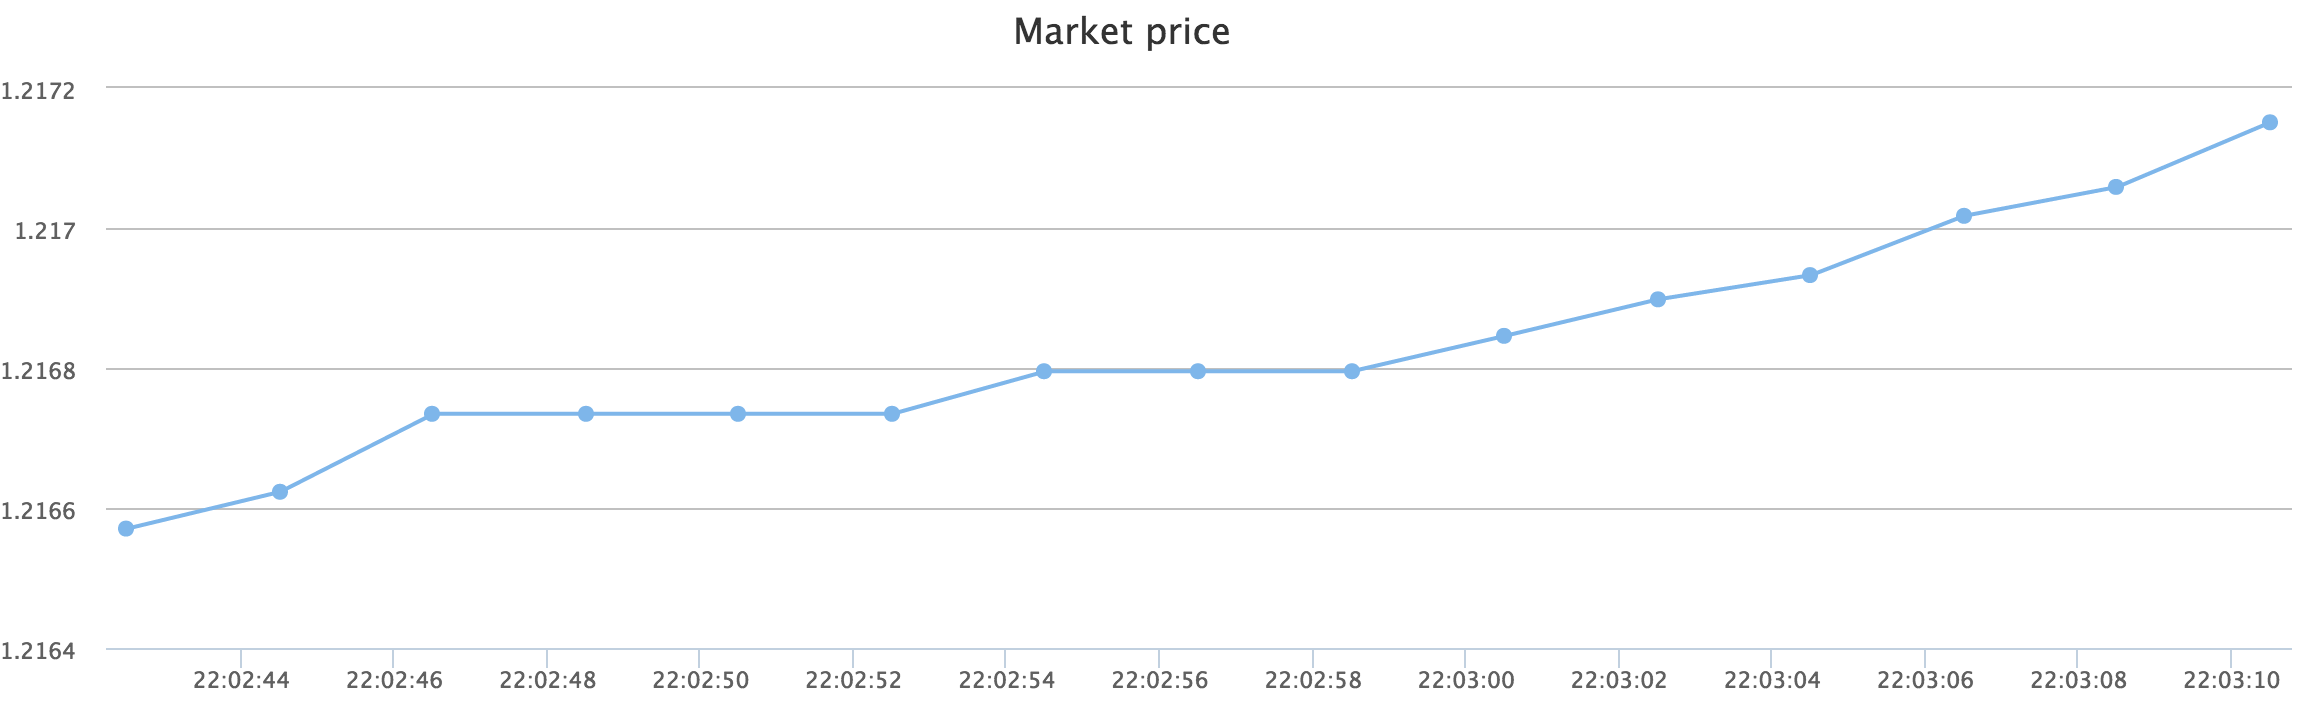
\includegraphics[width=0.9\textwidth]{img/examples/simulation-mad-buys-mm-sells.png} 
\label{fig:mm-sells}
\caption{Rising ask price due to market maker's spread in a buyers-only market.}
\end{figure}

Figure~\ref{fig:mm-buys} illustrates the counter-experiment. It shows price development
in a market where all agents are only allowed to place ask orders and the market maker 
is to buy all the offers. Consequently, the price monotonically decreases.

\begin{figure}[h]
\center
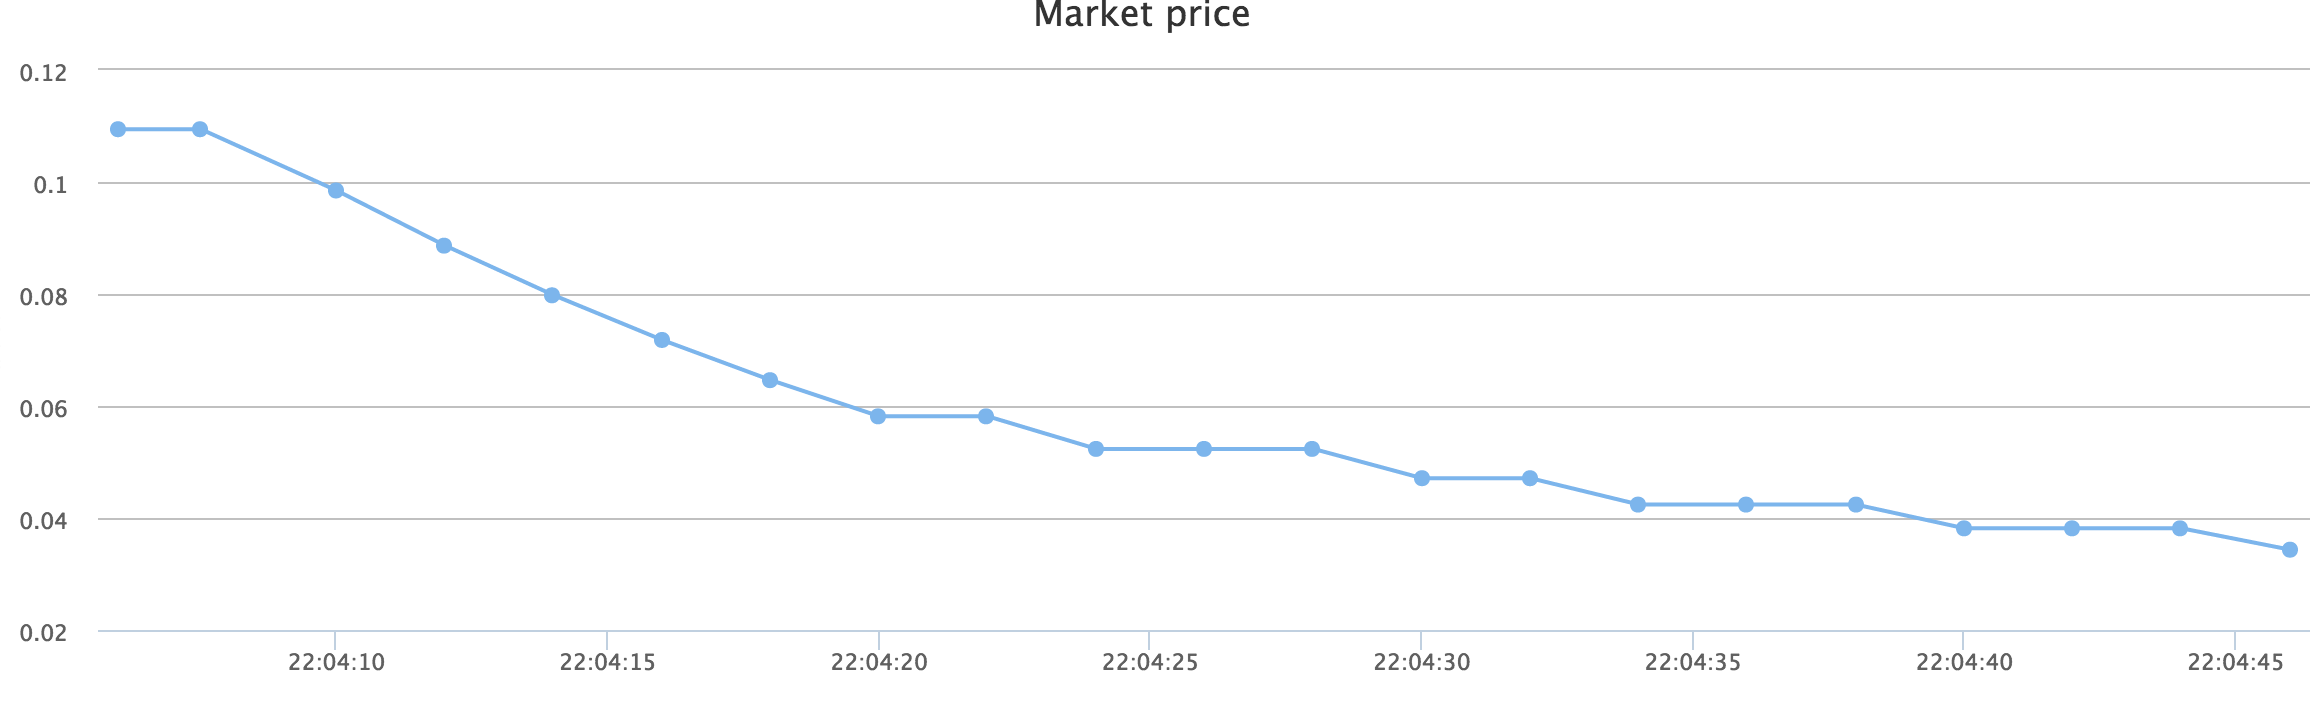
\includegraphics[width=0.9\textwidth]{img/examples/simulation-mad-sells-mm-buys.png} 
\label{fig:mm-buys}
\caption{Falling bid price due to market maker's spread in a sellers-only market.}
\end{figure}

In a market where agents are allowed to place any type of order, the price may oscillate
and is defined by demand and offer within the system (see Figure~\ref{fig:both}). 
Still, there might occur situations where the market maker has impact due to a lack of
bid or ask orders as can be seen in the left and right part of the figure.

\begin{figure}[h]
\center
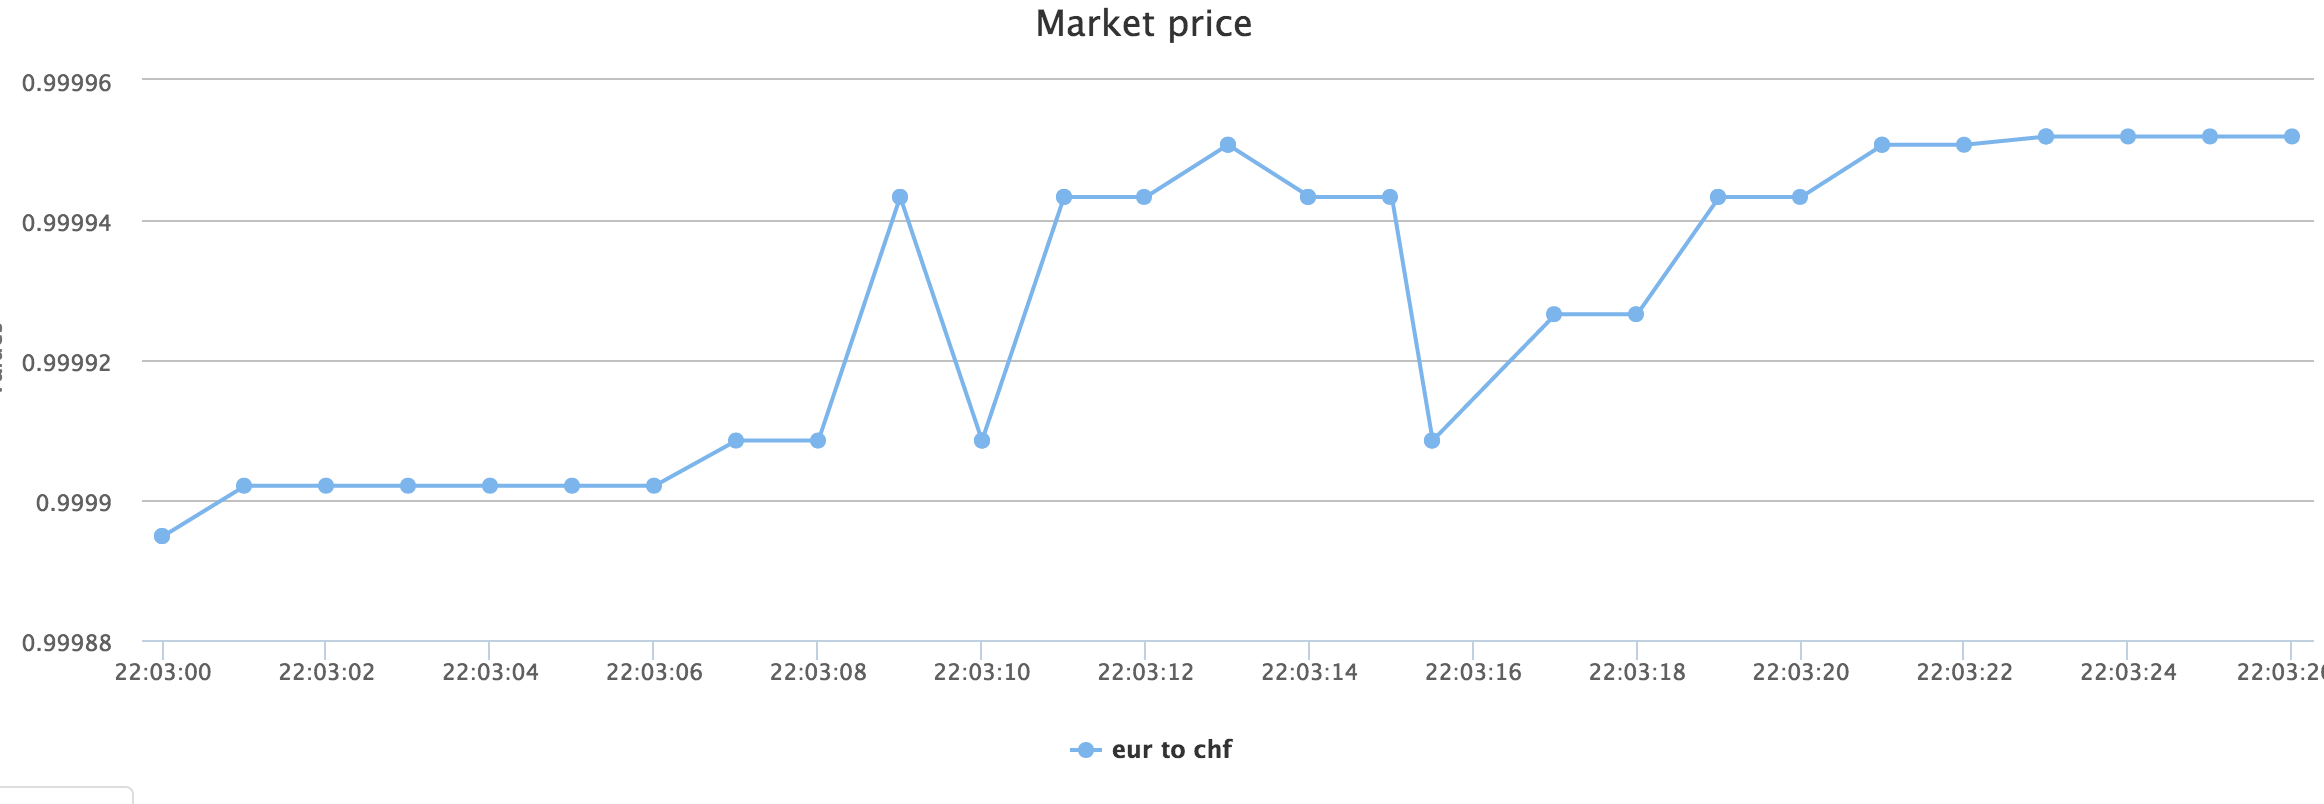
\includegraphics[width=0.9\textwidth]{img/examples/simulation-sell-and-buy.png} 
\label{fig:both}
\caption{Oscillating ask price in a full market simulation.}
\end{figure}

\subsection{Outline}
The software developed in this project is designed in a modular way. Hence, it is open
to adding new strategies and components. Extending the latter is particularly 
promising since the complexity of a real market is by far not fully covered yet. The next
important components are central banks. Since they fix interest rates on currencies 
they function as important indicators for strategies. Continuously implementing more
real actors will make the simulation more realistic and bring it closer to the goal 
of reflecting the actual market.

\subsection{Outline}
The software developed in this project is designed in a modular way. Hence, it is open
to adding new strategies and components. Extending the latter is particularly
promising since the complexity of a real market is by far not fully covered yet. The next
important components are central banks. Since they fix interest rates on currencies
they function as important indicators for strategies. Continuously implementing more
real actors will make the simulation more realistic and bring it closer to the goal
of reflecting the actual market.


%
%\subsection{Brain Storm}
%
%Market Simulation Research
%
%[1] http://www.tpc.org/tpc_documents_current_versions/pdf/tpce-v1.14.0.pdf
%[2] www.swissquote.com
%[3] http://vantagepointtrading.com/daily-forex-stats
%[4] http://www.bis.org/publ/qtrpdf/r_qt1312e.pdf
%[5] turnovers by counterparty and currency pairs:
%http://www.reuters.com/article/2013/09/05/bis-survey-volumes-idUSL6N0GZ34R20130905
%
%[6] largest forex centers:
%http://countingpips.com/fx/2011/08/8-largest-forex-trading-centers-in-the-world/
%
%[7] directional trading volume:
%http://www.dailyfx.com/forex/technical/article/special_report/2015/04/13/forex-introducing-volume-by-price.html
%
%[8] https://mahifx.com/blog/50-fascinating-facts-about-forex
%
%[9] largest brokers by volume:
%http://www.myfxbook.com/forex-broker-volume
%
%[10] volume survey (North America) with explanation
%http://www.newyorkfed.org/fxc/volumesurvey/explanatory_notes.html
%
%[11] forex glossary
%http://www.cmsfx.com/en/forex-education/Forex-Glossary/ask-price/
%
%[12] salary distribution switzerland
%http://www.bfs.admin.ch/bfs/portal/en/index/themen/03/04/blank/key/lohnstruktur/lohnverteilung.html
%
%[13] explanation of market makers
%http://www.forextraders.com/market-maker-forex-brokers.html
%
%p.47
%- Entity Relationships
%- Trade Types
%- run historical data for 300 business days before simulation starts
%
%Wanted:
%- trader initial funds -> half of annual income according to [12]?
%- broker initial funds (for leverage trades)
%- market maker funds
%- number of traders per currency pair
%- one market maker per currency pair?

